% Standalone source for Fig 1 (MI-Workbench architecture and review cycle).
% Build:  pdflatex Fig1.tex   ->  Fig1.pdf
% TIFF:   pdftoppm -r 600 -singlefile -tiff -tiffcompression lzw Fig1.pdf Fig1
% (see scripts/make_plos_figures.sh)
\documentclass[border=4pt]{standalone}
\usepackage[T1]{fontenc}
\usepackage[scaled]{helvet}
\renewcommand{\familydefault}{\sfdefault}
\usepackage{tikz}
\usetikzlibrary{arrows.meta,positioning,fit,calc,backgrounds}
\begin{document}
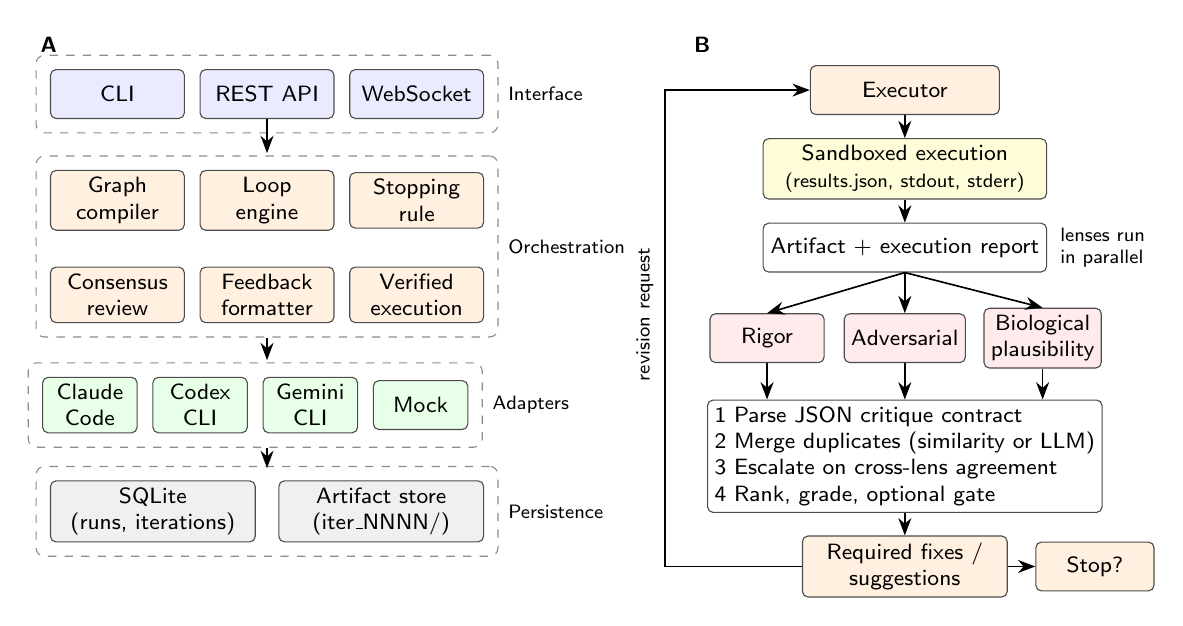
\begin{tikzpicture}[
  font=\sffamily\footnotesize,
  box/.style={rectangle, draw=black!70, rounded corners=2pt, minimum height=0.62cm, align=center, inner sep=2.5pt},
  layer/.style={rectangle, draw=black!45, dashed, rounded corners=3pt, inner sep=5pt},
  lab/.style={font=\sffamily\footnotesize\bfseries, anchor=north west},
  arr/.style={-{Stealth[length=2.2mm]}, semithick},
]
% ---------------- Panel A: layers ----------------
\node[lab] at (-0.2, 9.15) {A};
\node[box, fill=blue!8, minimum width=1.7cm] (cli) at (0.9, 8.3) {CLI};
\node[box, fill=blue!8, minimum width=1.7cm] (api) at (2.8, 8.3) {REST API};
\node[box, fill=blue!8, minimum width=1.7cm] (ws)  at (4.7, 8.3) {WebSocket};
\node[layer, fit=(cli)(ws), label={[font=\sffamily\scriptsize]right:Interface}] (L1) {};

\node[box, fill=orange!12, minimum width=1.7cm] (dsl)  at (0.9, 6.95) {Graph\\compiler};
\node[box, fill=orange!12, minimum width=1.7cm] (eng)  at (2.8, 6.95) {Loop\\engine};
\node[box, fill=orange!12, minimum width=1.7cm] (stop) at (4.7, 6.95) {Stopping\\rule};
\node[box, fill=orange!12, minimum width=1.7cm] (cons) at (0.9, 5.75) {Consensus\\review};
\node[box, fill=orange!12, minimum width=1.7cm] (fb)   at (2.8, 5.75) {Feedback\\formatter};
\node[box, fill=orange!12, minimum width=1.7cm] (exec) at (4.7, 5.75) {Verified\\execution};
\node[layer, fit=(dsl)(exec), label={[font=\sffamily\scriptsize]right:Orchestration}] (L2) {};

\node[box, fill=green!9, minimum width=1.2cm] (cl) at (0.55, 4.35) {Claude\\Code};
\node[box, fill=green!9, minimum width=1.2cm] (cx) at (1.95, 4.35) {Codex\\CLI};
\node[box, fill=green!9, minimum width=1.2cm] (gm) at (3.35, 4.35) {Gemini\\CLI};
\node[box, fill=green!9, minimum width=1.2cm] (mk) at (4.75, 4.35) {Mock};
\node[layer, fit=(cl)(mk), label={[font=\sffamily\scriptsize]right:Adapters}] (L3) {};

\node[box, fill=black!6, minimum width=2.6cm] (db) at (1.35, 3.0) {SQLite\\(runs, iterations)};
\node[box, fill=black!6, minimum width=2.6cm] (fs) at (4.25, 3.0) {Artifact store\\(iter\_NNNN/)};
\node[layer, fit=(db)(fs), label={[font=\sffamily\scriptsize]right:Persistence}] (L4) {};

\draw[arr] (2.8,7.98) -- (2.8,7.55);
\draw[arr] (2.8,5.2) -- (2.8,4.92);
\draw[arr] (2.8,3.8) -- (2.8,3.55);

% ---------------- Panel B: one review cycle ----------------
\begin{scope}[xshift=8.3cm]
\node[lab] at (-0.2, 9.15) {B};
\node[box, fill=orange!12, minimum width=2.4cm] (ex) at (2.6, 8.35) {Executor};
\node[box, fill=yellow!15, minimum width=3.6cm] (sb) at (2.6, 7.35) {Sandboxed execution\\{\scriptsize (results.json, stdout, stderr)}};
\node[box, fill=white, minimum width=3.6cm] (art) at (2.6, 6.35) {Artifact + execution report};
\node[box, fill=red!8, minimum width=1.45cm] (r1) at (0.85, 5.2) {Rigor};
\node[box, fill=red!8, minimum width=1.45cm] (r2) at (2.6, 5.2) {Adversarial};
\node[box, fill=red!8, minimum width=1.45cm] (r3) at (4.35, 5.2) {Biological\\plausibility};
\node[box, fill=white, minimum width=4.9cm, align=left] (mg) at (2.6, 3.7) {%
  1 Parse JSON critique contract\\
  2 Merge duplicates (similarity or LLM)\\
  3 Escalate on cross-lens agreement\\
  4 Rank, grade, optional gate};
\node[box, fill=orange!12, minimum width=2.6cm] (fd) at (2.6, 2.3) {Required fixes /\\suggestions};
\node[box, fill=orange!12, minimum width=1.5cm, right=0.35cm of fd] (sr) {Stop?};

\draw[arr] (ex) -- (sb);
\draw[arr] (sb) -- (art);
\draw[arr] (art.south) -- (r1.north);
\draw[arr] (art.south) -- (r2.north);
\draw[arr] (art.south) -- (r3.north);
\draw[arr] (r1.south) -- (mg.north -| r1);
\draw[arr] (r2.south) -- (mg.north);
\draw[arr] (r3.south) -- (mg.north -| r3);
\draw[arr] (mg) -- (fd);
\draw[arr] (fd) -- (sr);
\draw[arr] (fd.west) -- (-0.45,2.3) |- (ex.west);
\node[font=\sffamily\scriptsize, align=center, rotate=90] at (-0.7, 5.5) {revision request};
\node[font=\sffamily\scriptsize, anchor=west, align=left] at (4.45, 6.35) {lenses run\\in parallel};
\end{scope}
\end{tikzpicture}
\end{document}
